\subsection{Program Structure}
As mentioned our server is written in F\Sh which is a very powerful functional programming language with Types and parallel programming abilities. F\Sh can even be object oriented, but we have chosen not to use these abilities: We wanted the exercise of writing a fully functional system.

Our system is build of modules which are put together like bricks into layers that create a great structure.
\\We have an Outer Layer - or shell - which is the published Web Service. This layer is actually written in C\Sh.
\\Then we have a Checking Layer which uses a Permission Module to verify users and permissions before invoking functions deeper.
\\The Application Logic Layer is the actual working layer which has Account Module Product Module and more.
\\The Persistence Layer is the lowest logical layer. It has the responsibility to create, save and update information on some sort of data storage.
\\Finally we have our Database in which we store our data.

Each Module can be replaced and the Checking Layer is entirely optional. For example one might want to change the Persistence Layer to persist against a file-system instead of a database, or one might want to do less or more extensive checks in the Checking Layer, without changing any of the other layers.

\paragraph{Outer Layer}
\paragraph{Checking Layer}
\paragraph{Application Logic Layer}
\paragraph{Persistence Layer}

\begin{figure}[t]
  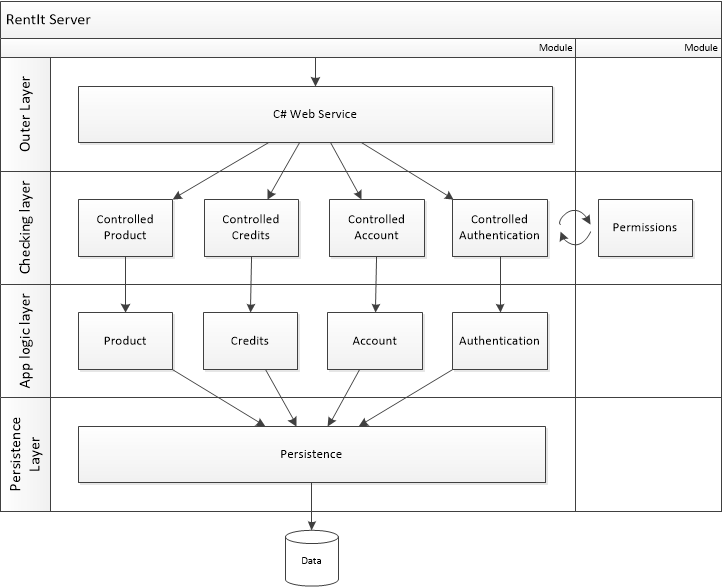
\includegraphics[width=\textwidth]{illustrations/ServerStructure.png}
  \caption{Our Server Structure}
  \label{fig:serverstructure}
\end{figure}

\subsubsection{Patterns Applied}
\newpage